\documentclass[12pt]{article}
	
%______________________PREAMBULO_________________________

%----------------------Paquetes--------------------------
\usepackage{amsmath,amssymb,amsfonts,latexsym,cancel} % Paquetes de símbolos adicionales.
\usepackage[spanish,es-tabla]{babel} % Idioma español
\usepackage[utf8]{inputenc} % Paquete que nos permite usar los acentos y otros símbolos, directamente del teclado.
\usepackage[T1]{fontenc} % Cambia el tipo de letra
\usepackage{times} % Tipo de letra Times New Roman
\usepackage{graphicx} % Paquete para el manejo de gráficos y figuras en el documento.
\usepackage{geometry} % Permite el manejo de los margenes
\usepackage{fancyhdr} % Permite colocar y manejar el encabezado
\usepackage[breaklinks,colorlinks=true,linkcolor=black,citecolor=blue, urlcolor=blue]{hyperref} % Crea hipervinculo entre secciones y el indice
\usepackage{pstricks}
\usepackage{float}
\usepackage{bm}
%\usepackage{multicol}
%\usepackage{mathpazo} %fuente palatino
%\usepackage{xcolor}
%\usepackage[shortlabels]{enumitem}
%-------------Paquetes para el formato de las citas-------
%\usepackage[hyphens]{url}
%\usepackage{cite}
%\usepackage{wrapfig}

%-----------------------------ayuda de paquetes--------------------

\spanishdecimal{.}
\providecommand{\abs}[1]{\lvert#1\rvert}

%------------------------Margenes----------------------------

\newgeometry{bottom = 2.5 cm, top = 2.5 cm, left = 2 cm, right = 2 cm} % Modifica el margen {Abajo, Arriba, Izquierda, Derecha

%----------------------------Interlineado----------------------------------

%\doublespacing
%\onehalfspace
%\singlespace
%\spacing{1.5} % Permite personalisar a gusto
%\setlength{\parskip}{2cm} % Es el espacio entre parrafos

%-----------------------------Sangria---------------------------------------

\setlength{\parindent}{0 cm} % Manipula la sangria

%---------------------Portada------------------

%\title{
%\begin{figure}[h!]
		
%	\centering
%	
\includegraphics[width=\linewidth]{Nom_UAdeC_FCFM.png}  			
			
%\end{figure}
%\huge \textbf{LABORATORIO DE FISICA 3}\\\LARGE TITULO PRACTICA\\}
%\author{ \Large \textbf{Profesor:}\\
%\Large \textbf{Alumno:} Oscar Joel Castro Contreras}
%\date{\today}

%--------------Encabezado y pie de pagina--------------------

\pagestyle{fancy}%Coloca el encabezado en el documento
\lhead[]{Métodos numéricos}%Encabezado izquierda
\rhead[]{Oscar Joel Castro Contreras}%Encabesado derecha
%\chead[]{}%Encabesado central
\renewcommand{\headrulewidth}{0.08 pt}%Coloca linea al pie de pagina

%\lfoot[]{PI}%Pie de pagina izquerdo
%\rfoot[]{PD}%Pie de pagina derecho
\cfoot[]{\thepage}%Pie de pagina central
\renewcommand{\footrulewidth}{0.08 pt}%Coloca linea al pie de pagina

%-----------------------------------------------------------------------------

	\begin{document}
		
		\begin{titlepage}
		
			\centering
			{\bfseries
			\begin{figure}[h!]
				\centering
				
\includegraphics[width=\linewidth]{Nom_UAdeC_FCFM.png} 				
			\end{figure}
			\par}
			\vspace{2cm}
			{\scshape\LARGE Métodos numéricos \par}
			\vspace{3cm}
			{\scshape\Huge \textbf{Método de bisección} \par}
			\vfill
			{\LARGE \textbf{Profesora:} Maria Guadalupe Godina Cubillo \par}
			\vspace{3cm}
			{\LARGE \textbf{Alumno:} Oscar Joel Castro Contreras \par}
			\vfill
			{\Large \today \par}
			\thispagestyle{empty}
			%\thispagestyle{fancy}
			
		\end{titlepage}
	
		\newpage

		\begin{abstract}
			\noindent En este reporte explico un poco de los métodos que existen para encontrar las raíces de cualquier 
			polinomio o función que tenga raíces, y en específico explico, qué es, en que consiste y cuales son las 
			limitaciones del método de bisección para encontrar raíces.
		\end{abstract}

		\textbf{Palabras clave:} Raíces, Bisección, Valor Intermedio, Tolerancia.

		\section*{\centering Introducción}\label{sec:Introducción}
			Los polinomios son uno de los conceptos más importantes en álgebra y son fundamentales en 
			matemáticas y ciencia en general. Determinar las raíces de un polinomio es uno de los problemas 
			más antiguos en matemáticas.\\
			Puesto que las ecuaciones polinomiales aparecen en un amplio rango de áreas de la ciencia, desde 
			química y física básica hasta economía, el problema de determinar raíces de polinomios es, con 
			frecuencia, un paso obligado en la resolución de problemas.\cite{bib:item1}\\
			La razón principal para resolver ecuaciones no lineales por medio de métodos computacionales es 
			que algunas ecuaciones carecen de solución exacta, excepto por unas pocas. Por lo que existen 
			métodos numéricos diseñados para obtener las raíces, aunque cada uno tiene sus propias 
			limitaciones y defectos. Algunos métodos se muestran en la tabla \ref{tab:1}\cite{bib:item2}\\
			\begin{table}[h!]
				\centering
				\begin{tabular}{|c|c|}
					\hline
					\multicolumn{2}{|c|}{\textbf{Métodos numéricos para obtener raíces}}\\
					\hline
					\textbf{Nombre} & \textbf{Características} \\\hline
					Bisección & Aplicable a funciones no analiticas \\\hline
					Falsa posición & Convergencia lenta en un intervalo grande \\\hline								
					Método de Newton & Rápido, se nesecita calcular derivada \\\hline
					Método de secante & Rápido, no se requiera calcular derivada \\\hline
					Sustitución sucesiva & Puede no converger \\\hline
				\end{tabular}
				\caption{Métodos numéricos para obtener raíces \cite{bib:item2}}
				\label{tab:1}
			\end{table}\\
			En general, no es posible determinar los ceros de una función, es decir, valores $ x^* $ tal que $f(x^*) = 0 $, 
			en un número finito de pasos. Tenemos que usar métodos de aproximación. Los métodos son 
			usualmente iterativos y tienen la forma: Iniciando con una aproximación inicial $ x_0 $ (o un intervalo $ [a,b] $) , 
			se calculan aproximaciones sucesivas $ x_1,x_2,... $ y elegimos $ x_n $ como aproximación de $ x^* $ cuando se cumpla un 
			criterio de parada dado. A los ceros de un polinomio se les conoce también como raíces. \cite{bib:item3} \\
			\textbf{El método de Bisección:}\\	
			Este es uno de los métodos más sencillos y de fácil intuición, para resolver ecuaciones en una 
			variable. Se basa en el Teorema de los Valores Intermedios, el cual establece que toda función 
			continua $ f $ en un intervalo cerrado $ [a,b] $ en el que se encuentra la raíz, toma todos los valores que se 
			hallan entre $ f(a) $ y $ f(b) $. Esto es, que todo valor entre $f(a) $ y $ f(b) $ es la imagen de al menos un valor 
			en el intervalo $ [a,b] $.\\
			En caso de que $ f(a) $ y $ f(b) $ tengan signos opuestos, es decir, $ f(a)f(b) < 0 $, el valor cero sería un 
			valor intermedio entre $ f(a) $ y $ f(b) $, por lo que con certeza existe un $ x^* $ en $ [a,b] $ que cumple $f(x^*) = 0 $. 
			De esta forma, se asegura la existencia de al menos una solución de la ecuación $ f(x) = 0 $. \cite{bib:item2}
		\section*{\centering Metodología}\label{sec:Metodologia}
			El método consiste en suponer que tengamos un intervalo $ [a,b] $ donde esta una raíz de la función $ f(x) $. 
			Primero evaluamos la función en los intervalos y verificamos $$ f(a)f(b) < 0 $$ si esto no se 
			cumple el método no funcionara, después de verificar que lo anterior se cumple, debemos calculamos el punto 
			medio del intervalo $ [a,b] $. $$ x_m = \frac{a+b}{2},\text{ donde para reducir el error en el código se uso } x_m = b+\frac{a-b}{2} $$
			Después calculamos $ f(x_m) $. En caso de que $ f(x_m) = 0 $, ya hemos encontrado la raíz. Pero en 
			caso de que no lo sea, ahora la raíz se encuentra entre $ [a,x_m] $ o $ [x_m,b] $. para poder determinar 
			a cuál de los 2 intervalos pertenece la raíz, hay que verificar $$ f(a)f(x_m) > 0 $$ si esto se 
			cumple, entonces, la raíz se encuentra en $ [a,x_m] $, si no se cumple ahora, hay que verificar $$ f(b)f(x_m) > 0 $$ si esto se cumple, 
			entonces, la raíz se encuentra en $ [x_m,b] $. Ahora repetimos todo el proceso, pero con el intervalo 
			que obtuvimos. Así vamos interando y reduciendo el intervalo la veces necesarias para encontrar la mejor 
			aproximación al raíz de la función $ f(x) $.\\
			El criterio para parar las interacciones esta dado por el numero de cifras significativas que queramos, 
			de aquí obtenemos una tolerancia, la cual en cada interacción se compara con el error relativo y 
			absoluto, si uno de los errores es menor o igual a la tolerancia, detener las interacciones. De todo 
			esto surge una ecuación que nos permite determinar el número exacto de interacciones, para 
			aproximarnos a la raíz una cierta cantidad de cifras significativas. La ecuación es $$ n = \frac{\log{\abs{b-a}}-\log{\abs{tol}}}{\log{\abs{2}}} $$

		\section*{\centering Resultado}\label{sec:Resultado}
			En esta parte de mi programa se calcula la tolerancia para las determinar el número interacciones que se realizaran.
			\begin{center}
				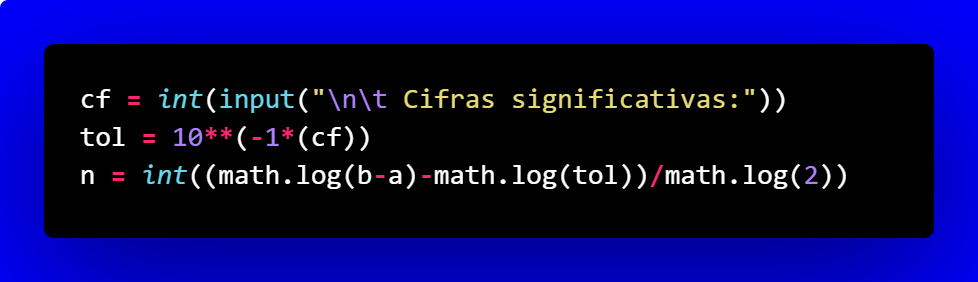
\includegraphics[width=\linewidth]{Figura 1.png} 				
			\end{center}
			Esta parte calcula el valor medio entre el intervalo $ [a.b] $, con la ecuación $ x_m = b+\frac{a-b}{2} $.
			\begin{center}
				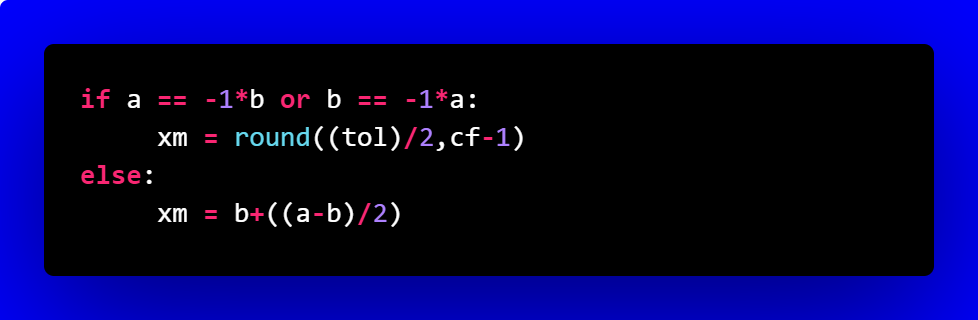
\includegraphics[width=\linewidth]{Figura 2.png} 				
			\end{center}
			Esta parte define cual será el siguiente intervalo en el que se calculará el valor medio.
			\begin{center}
				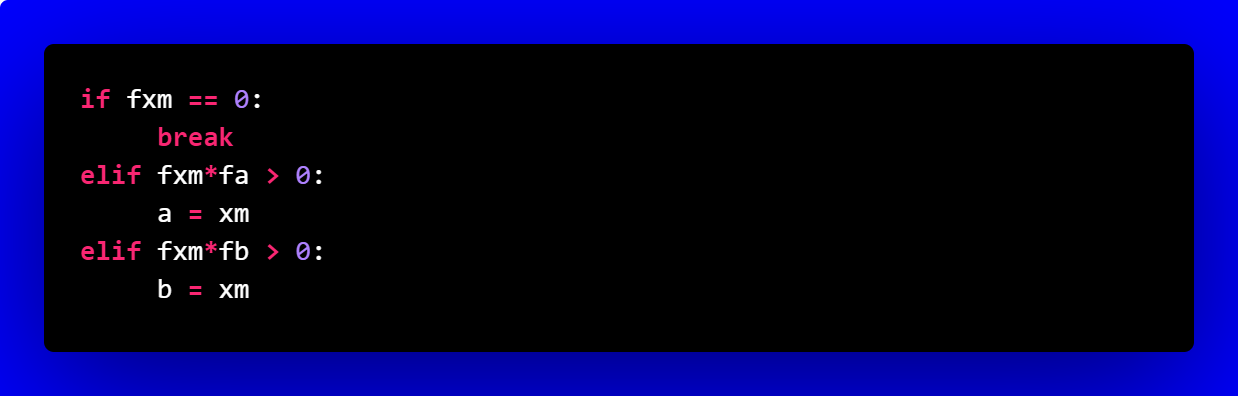
\includegraphics[width=\linewidth]{Figura 3.png} 				
			\end{center}
		
		\section*{\centering Observación}\label{sec:Observacion}
			Si regresamos a la condición inicial de que $$ f(a)f(b) < 0 $$
			si esta condición no se cumple, el método no funciona para esa función, este es una de las 
			limitaciones del método, esto ocurre en diferentes situaciones.\\
			La condicion no se cumple cuando:
			\begin{itemize}
				\item En el intevalo $ [a,b] $, no hay la raícas, de la función.
				\item La funcion no tiene raíces reales,
				\item Hay mas de 1 raiz en el intervalo $ [a,b] $ dado.
				\item En general cuando la evaluación de $ f(a) $ tiene el mismo signo que $ f(b) $.
			\end{itemize}
		

		\section*{\centering Conclusión}\label{sec:Conclusion}
			En conclusión, el método de bisección permite encontrar la raíz aproximada de una función a partir 
			de un intervalo $ [a,b] $ en el que este la raíz de la función, con el teorema de los valores intermedios. 
			Esto lo puede realizar siempre y cuando se cumpla la condicione de que $ f(a)f(b) < 0 $ ya que, si esta condición no 
			se cumple, puede que dentro del intervalo no existe ninguna raíz, que la función no tenga raíces 
			reales o que halla mas de una raíz en el intervalo. Solo para estas condiciones especiales este 
			método de bisección no funciona.

		\centering
		\begin{thebibliography}{10}
			\bibitem{bib:item1} de la Vega, H. M. El calculo de raıces de polinomios. Una historia sin fin. Recuperado de
							\href{http://www.matedu.cinvestav.mx/~elcalculoysuensenanza/investigacion/articulosPDF/Madrid.pdf}{Pagina web de \cite{bib:item1}}.
			\bibitem{bib:item2} Nakamura, S. (1998). Metodos Numericos Aplicados Con Software. En Solución de ecuaciones no lineales (Primera ed., pp. 62–63). Prentice Hall.
			\bibitem{bib:item3} Mora, W. (2010). Introducción a los Métodos Numéricos. Implementaciones en R. Ecuaciones no lineales (Primera ed., pp. 95,110) Recuperado de
							\href{https://tecdigital.tec.ac.cr/revistamatematica/Libros/WMora_MetodosNumericos/2017_Principal_MetodosNumericos-con-R.pdf}{Pagina web de \cite{bib:item3}}. 
							
			
		\end{thebibliography}

	\end{document}